
\chapter{Literature Review} 

In induction machine, a power converter and a controller are the three major components of an induction motor drive system. Some of the disciplines related to these components are electric machine design, electric machine modeling, sensing and measurement techniques, signal processing, power electronic design and electric machine control. It is beyond the scope of this research to address all of these areas: it will primarily focus on the issue related to the induction machine control. A conventional low cost volts per hertz or a high performance field oriented controller can be used to control the machine. This chapter reviews the principles of the field orientation control of the induction machines and outline major problems in its design and implementation.


\section{Induction machine control}

The controllers required for induction motor drives can be divided into two major types: a conventional low cost volts per hertz v/f controller and torque controller \cite{Vas}-\cite{Lipo}. In v/f control, the magnitudes of the voltage and frequency are kept in proportion. The performance of the v/f control is not satisfactory, because the rate of change of voltage and frequency has to be low. A sudden acceleration or deceleration of the voltage and frequency can cause a transient change in the current, which can result in drastic problems. Some efforts were made to improve v/f control performance, but none of these improvements could yield a v/f torque controlled drive systems and this made DC motors a prominent choice for variable speed applications. This began to change when the theory of field orientation was introduced by Hasse and Blaschke. Field orientation control is considerably more complicated than DC motor control. The most popular class of the successful controllers uses the vector control technique because it controls both the amplitude and phase of AC excitation. This technique results in an orthogonal spatial orientation of the electromagnetic field and torque, commonly known as Field Oriented Control (FOC).


\section{Field orientation control (FOC) of induction machine}


The concept of field orientation control is used to accomplish a decoupled control of flux and torque. This concept is identical to a dc machine direct torque control that has following requirements \cite{Lipo}:
\begin{itemize}
\item{An independent control of armature current to overcome the effects of armature winding resistance, leakage inductance and induced voltage}
\item{An independent control of constant value of flux}
\end{itemize}

If all of these requirements are met at every instant of time, the torque will follow the current, allowing an immediate torque control and decoupled flux and torque regulation.\\

Next, a two phase d-q model of an induction machine rotating at the synchronous speed is introduced which will help to carry out this decoupled control concept to the induction machine. This model can be summarized by the following equations (see chapter 4 for detail):

\begin{align}
V_{ds}^{\omega}&=R_{s}i_{ds}^{\omega}+\frac{d}{dt}\psi_{ds}^{\omega}-\omega_{e}\psi_{qs}^{\omega}\\
V_{qs}^{\omega}&=R_{s}i_{qs}^{\omega}+\frac{d}{dt}\psi_{qs}^{\omega}+\omega_{e}\psi_{qs}^{\omega}\\
0&=R_{r}i_{dr}^{\omega}+\frac{d}{dt}\psi{dr}^{\omega}-(\omega_{e}-\omega_{r})\psi_{qr}^{\omega}\\
0&=R_{r}i_{qr}^{\omega}+\frac{d}{dt}\psi{qr}^{\omega}+(\omega_{e}-\omega_{r})\psi_{dr}^{\omega}\\
T_{e}&=3p\frac{L_{m}}{L_{r}}(\psi_{dr}^{\omega}i_{qs}^{\omega}-\psi_{qr}^{\omega}i_{ds}^{\omega})
\end{align}

\begin{figure}[h]
\centering
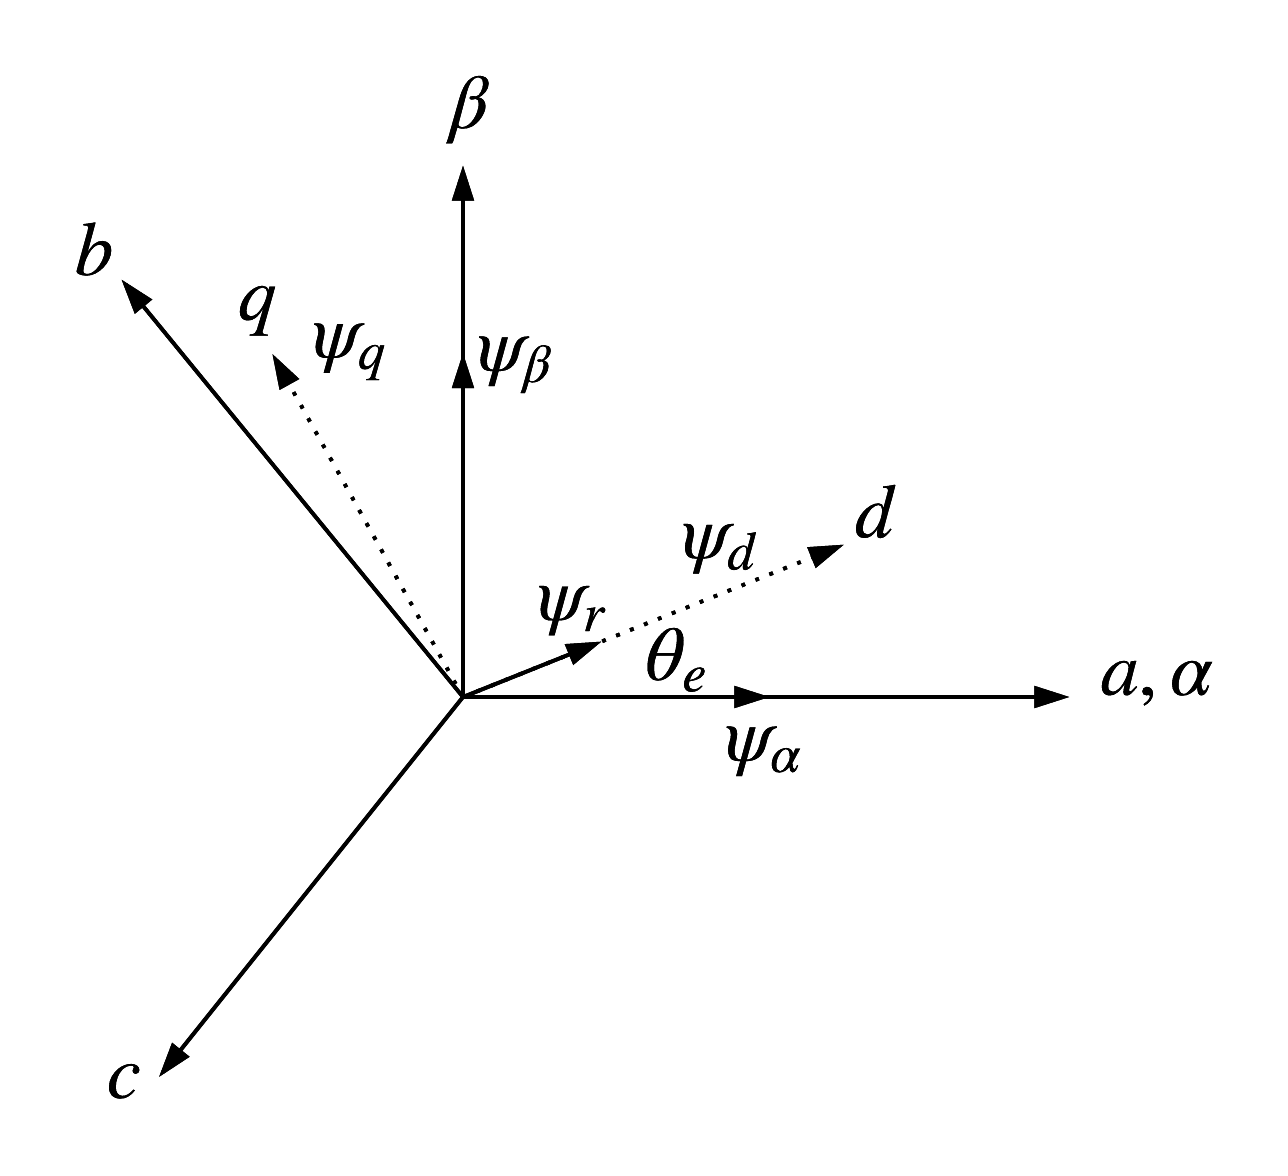
\includegraphics[scale=0.65]{chapter0/phasordig}
\caption{Phasor diagram of the field oriented drive system}
\label{phasor}
\end{figure}

and it is quite significant to synthesize the concept of field-oriented control. In this model it can be seen from the torque expression (2.5) that, if the flux along the q-axis
can be made zero then all the flux is aligned along the d-axis and, therefore, the torque can be instantaneously controlled by controlling the current along q-axis. Then the question will be how it can be guaranteed that all the flux is aligned along the d-axis of the machine. When three-phase voltages are applied to the machine, they produce three-phase fluxes both in the stator and the rotor. The three phase fluxes can be represented in a two phase stationary ($\alpha$-$\beta$) frame. If these two phase fluxes along ($\alpha$-$\beta$) axes are represented by a single-vector then all the machine flux will be aligned along that vector. This vector is commonly specified as d-axis which makes an angle $\theta_{e}$ with the stationary frame $\alpha$-axis, as shown in \autoref{phasor}. The q-axis is set perpendicular to the d-axis. The flux along the q-axis in this case will be obviously zero. The phasor diagram \autoref{phasor} presents these axes. When the machine input currents change sinusoidally in time, the angle $\theta_{e}$ keeps changing. Thus the problem is to know the angle $\theta_{e}$ accurately, so that the d-axis of the d-q frame is locked with the flux vector.\\


The control inputs can be specified in two phase synchronously rotating d-q frame as $i_{ds}^{\omega}$ and $i_{qs}^{\omega}$ such that $i_{ds}^{\omega}$ being aligned with the d-axis or the flux vector. These two phase synchronous control inputs are converted into two phase stationary quantities and then to three phase stationary control inputs. To accomplish this the flux angle $\theta_{e}$ must be known precisely. The angle $\theta_{e}$ can be found either by Direct Field Orientation control (DFO) or by Indirect Field Orientation control (IFO). The controller implemented in this fashion that can achieve a decoupled control of the flux and the torque is known as field oriented controller. The block diagram is shown in the \autoref{foc} In the field-oriented controller the flux can be regulated in the stator, air-gap or rotor flux orientation \cite{Vas}-\cite{Lipo}.


\begin{figure}[h]
\centering
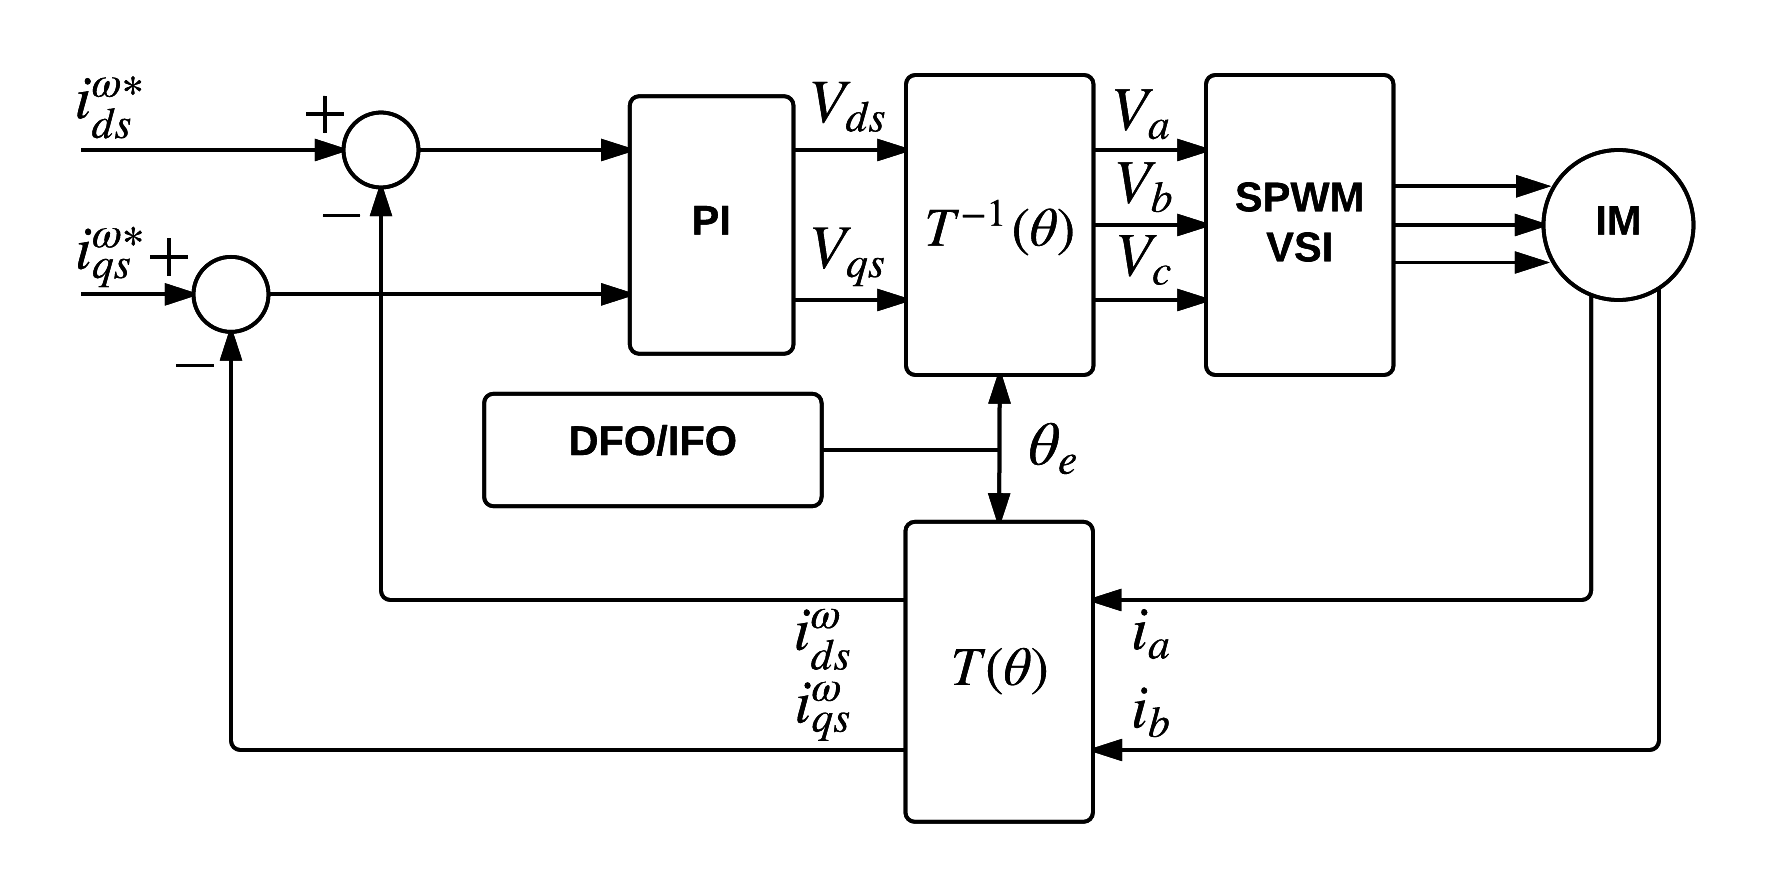
\includegraphics[scale=0.73]{chapter0/foc}
\caption{Field oriented induction motor drive system}
\label{foc}
\end{figure}

The control algorithm for calculation of the rotor flux angle $\theta_{e}$ using IFO control is shown in the \autoref{ifoc}. This algorithm is based on the assumption that, the flux along the q-axis is zero, which forces the command slip velocity to be $\omega_{sl}=i_{qs}^{\omega}/(\tau_{r}i_{ds}^{\omega})$ as a necessary and sufficient condition to guarantee that all the flux is aligned with d-axis and the flux along q-axis is zero. The angle $\theta_{e}$ can then be determined as the sum of the slip and the rotor angles after integrating the respective velocities. This slip angle includes the necessary and sufficient condition for decoupled control of flux and torque. The rotor speed can be measured directly by using an encoder or can be estimated. In case the rotor speed is estimated, the control technique is known as sensorless control. This concept will be studied in detail in the following chapters. \autoref{dfo} shows the control algorithm block diagram for DFO control. In this technique the flux angle $\theta_{e}$ is classically calculated by sensing the air-gap flux through the use of flux sensing coils, or can be calculated by estimating the flux along the d-q axes using the voltage and current signals.

\begin{figure}[h]
\centering
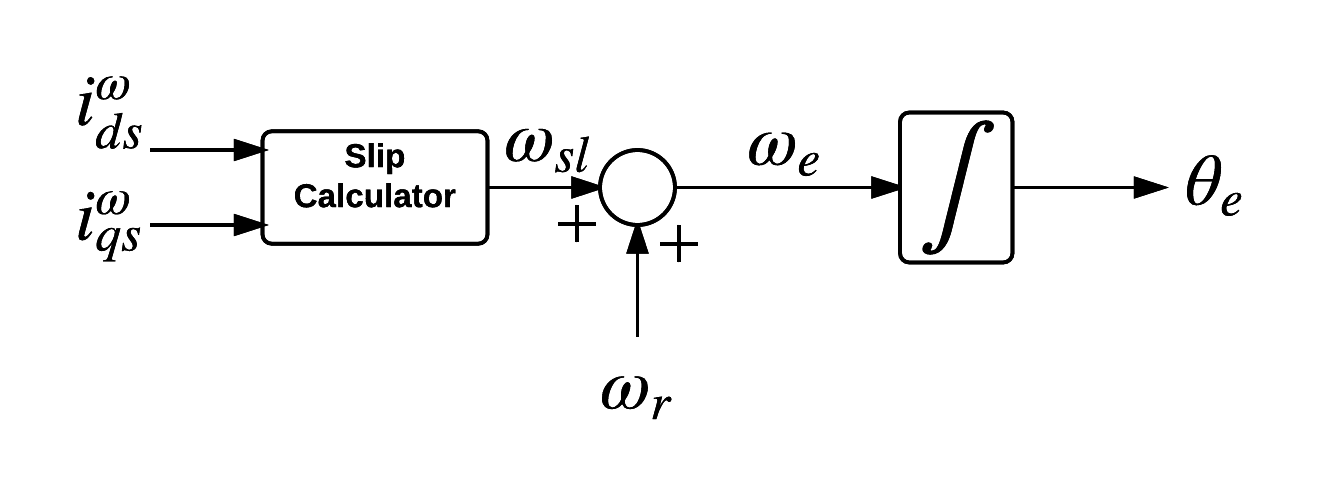
\includegraphics[scale=0.85]{chapter0/ifoc}
\caption{Indirect field oriented drive system}
\label{ifoc}
\end{figure}

\begin{figure}[h]
\centering
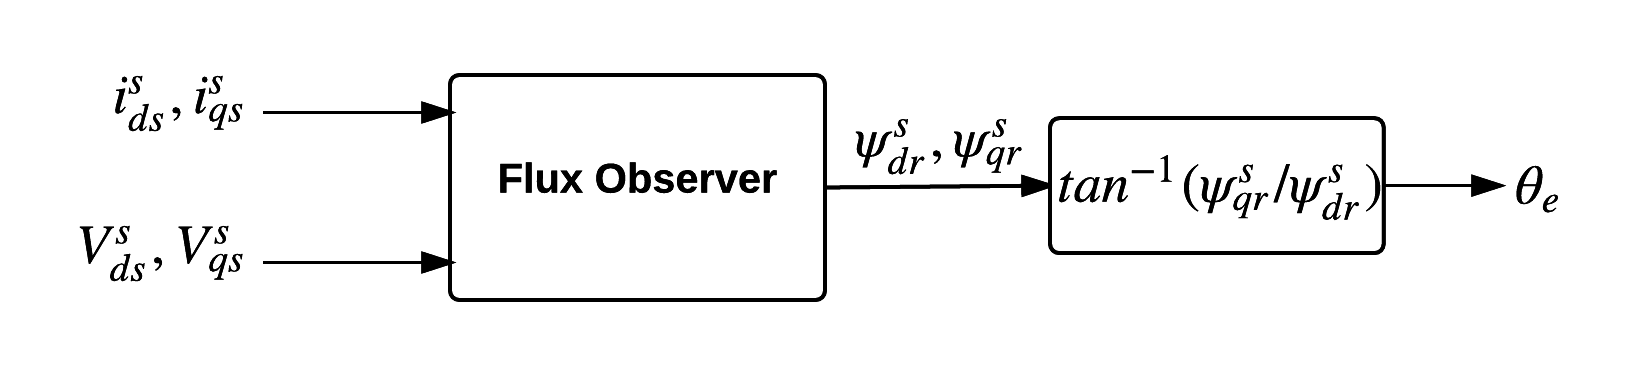
\includegraphics[scale=0.8]{chapter0/dfo}
\caption{Direct field oriented drive system}
\label{dfo}
\end{figure}

\subsection{Direct field orientation (DFO)}

The DFO control and sensorless control rely heavily on accurate flux estimation. DFOC is most often used for sensorless control, because the flux observer used to estimate the synchronous speed or angle can also be used to estimate the machine speed. Investigation of ways to estimate the flux and speed of the induction machine has also been extensively studied in the past two decades. Classically, the rotor flux was measured by using a special sensing element, such as Hall effect sensors placed in the air-gap. An advantage of this method is that additional required parameters, $L_{lr}$, $L_{m}$, and $L_{r}$ are not significantly affected by changes in temperature and flux level. However, the disadvantage of this method is that a flux sensor is expensive and needs special installation and maintenance. Another flux and speed estimation technique is saliency based with fundamental or high frequency signal injection. One advantage of saliency technique is that the saliency is not sensitive to actual motor parameters, but this method fails at low and zero speed level. When applied with high frequency signal injection \cite{jansen}, the method may cause torque ripples, and mechanical problems.\\

Gabriel \cite{Gabrie} avoided the special flux sensors and coils by estimating the rotor flux from the terminal quantities (stator voltages and currents). This technique requires the knowledge of the stator resistance along with the stator, rotor leakage inductances and magnetizing inductance. This method is commonly known as the Voltage Model Flux Observer (VMFO). The stator flux in the stationary frame estimated by the equations:


\begin{align}
\psi_{ds}^s&=V_{ds}^s-R_{s}i_{ds}^s\\
\psi_{qs}^s&=V_{qs}^s-R_{s}i_{qs}^s
\end{align}
Then the rotor flux can be expressed as:
\begin{align}
\psi_{dr}^s&=\frac{L_{r}}{L_{m}}(\psi_{ds}^s-\sigma i_{ds}^s)\\
\psi_{qr}^s&=\frac{L_{r}}{L_{m}}(\psi_{qs}^s-\sigma i_{qs}^s)
\end{align}

In this model, integration of the low frequency signals, dominance of stator resistance voltage drop at low speed and leakage inductance variation result in a less precise flux estimation. Integration at low frequency is studied by \cite{jun} and three different alternatives are given. Estimation of rotor flux from the terminal quantities depends on parameters such as stator resistance and leakage inductance. The study of parameter sensitivity shows that the leakage inductance can significantly affect the system performance such as stability, dynamic response, and utilizations of the machine and the inverter.\\


The Current Model Flux Observer (CMFO) is an alternative approach to overcome the problems of leakage inductance and stator resistance at low speed. In this model flux can be estimated as:
\begin{align}
\psi_{dr}^s=-\frac{1}{\tau_{r}}\psi_{dr}^s-\omega_{r}\psi_{qr}^s+\frac{L_{m}}{\tau_{r}}i_{ds}^s\\
\psi_{qr}^s=-\frac{1}{\tau_{r}}\psi_{qr}^s-\omega_{r}\psi_{dr}^s+\frac{L_{m}}{\tau_{r}}i_{qs}^s
\end{align}

However, it does not work well at high speed due to its sensitivity to the rotor resistance. Jansen \cite{pl} did an extensive study on VMFO and CMFO based direct field orientation control, discussed the design and accuracy assessment of various flux observers, compared them, and analyzed the alternative flux observers. To further improve the observer performance, closed-loop rotor flux observers are proposed which use the estimated stator current error \cite{pl,gc} or the estimated stator voltage error \cite{gc} to estimate the rotor flux. Furthermore, Lennart \cite{len} proposed reduced order observers for this task.

\subsection{Indirect field orientation control (IFOC)}


In indirect field orientation, the synchronous speed $\omega_{e}$ is the same as the instantaneous speed of the rotor flux vector $\psi_{dr}^{\omega}$ and the d-axis of the d-q coordinate system is exactly locked on the rotor flux vector (rotor flux vector orientation). This facilities the flux control through the magnetizing current $i_{ds}^{\omega}$ by aligning all the flux with the d-axis while aligning the torque producing component of the current with the q-axis. After decoupling the rotor flux and torque producing component of the current components, the torque can be instantaneously controlled by controlling the current $i_{qs}^{\omega}$. The requirement to align the rotor flux with the d-axis of the d-q coordinate system means that the flux along the q-axis must be zero. This means that the current through the q-axis of the mutual inductance is zero.\\

Based on this restriction $\omega_{sl}$ is :

\begin{align}
\omega_{sl}=\frac{i_{qs}^{\omega}}{(\tau_{r}i_{ds}^{\omega})}
\end{align}

These relations suggest that flux and torque can be controlled independently by specifying d-q axis currents provided the slip frequency is satisfied (2.12) at all instants.\\


The concept of indirect field oriented control developed in the past has been widely studied by researchers during the last two decades. The rotor flux orientation is both the original and usual choice for the indirect orientation control. Also the IFO control can be implemented in the stator and air-gap flux orientation as well. De Doncker \cite{doncker} introduced this concept in his universal field oriented controller. In the air-gap flux the slip and flux relations are coupled equations and the d-axis current does not independently control the flux as it does in the rotor flux orientation. For the constant air-gap flux orientation, the maximum of the produced torque is \%20 less than that of the other two methods \cite{sul}. In the stator flux orientation, the transient reactance is a coupling factor and it varies with the operating conditions of the machine. In addition, Mircea \cite{mirc} shows that among these methods, rotor flux oriented control has linear torque curve. Therefore, the most commonly used choice for IFO is the rotor flux orientation.\\

The IFOC is an open loop, feed forward control in which the slip frequency is fed forward guaranteeing the field orientation. This feed forward control is very sensitive to the rotor open circuit time constant $\tau_{r}$. Therefore, $\tau_{r}$ must be known in order to achieve a decoupled control of torque and flux components by controlling $i_{ds}^{\omega}$ and $i_{qs}^{\omega}$ , respectively. When $\tau_{r}$ is not set correctly, the machine is said to be detuned and the performance will become sluggish due to loss of decoupled control of torque and flux. The measurement of the rotor time constant, its effects on the system performance and its adaptive tuning to the variations resulting during the operation of the machine have been studied extensively in the literature \cite{rl}-\cite{krisn}. Lorenz, Krishnan and Novotny \cite{rl}-\cite{krisn} studied the effect of temperature and saturation level on the rotor time constant and concluded that it can reduce the torque capability of the machine and torque/amps of the machine. The detuning effect becomes more severe in the field-weakening region. Also, it results in a steady-state error and, transient oscillations in the rotor flux and torque. Some of the advanced control techniques such as estimation theory tools and adaptive control tools are also studied to estimate rotor time constant and other motor parameters \cite{ca}-\cite{jm}.\\


\section{Variable speed control using advance control algorithms}

There are two issues in motion control using field oriented controlled (FOC) induction machine drives. One is to make the resulting drive system and the controller robust against parameter deviations and disturbances. The other is to make the system intelligent to adjust the control system itself to environment changes and task requirements. If the speed regulation loop fails to produce the command current correctly, than the desired torque response will not be produced by the induction machine. In addition, such a failure may cause the degradation of slip command. As a result, a satisfactory speed regulation is extremely important not only to produce desired torque performance from the induction machine but also to guarantee the decoupling between control of torque and flux.\\

Conventionally, a PI controller has been used for the speed regulation to generate a command current for last two decades, and accepted by industry because of its simplicity. Even though, a well tuned PI controller performs satisfactorily for a field oriented induction machine during steady state. The speed response of the machine at transient, especially for the variable speed tracking, may sometimes be problematic. In last two decades, alternative control algorithms for the speed regulation were investigated. Among these, fuzzy logic, sliding mode, and adaptive nonlinear control algorithms gained much attention.\\

A traditional rotor flux oriented induction machine drive offers a better control performance but it often requires additional sensors on the machine. This adds to the cost and complexity of the drive system. To avoid these sensors on the machine, many different algorithms are proposed for the last three decades to estimate the rotor flux vector and rotor shaft speed. The recent trend in field oriented control is to use such algorithms based on the terminal quantities of the machine for the estimation of the fluxes and speed. They can easily be applied to any induction machine. Therefore, our focus in this study is also on these algorithms.\\


Before looking into individual approaches, the common problems of the speed and flux estimation are discussed briefly for general field orientation and state estimation algorithms.
 \begin{itemize}
 \item{\textbf{Parameter sensitivity:} One of the important problems of the sensorless control algorithms for the field oriented induction machine drives is the insufficient information about the machine parameters which yield the estimation of some machine parameters along with the sensorless structure. Among these parameters stator resistance, rotor resistance and rotor time constant play more important role than the other parameters since these values are more sensitive to temperature changes. The knowledge of the correct stator resistance $R_{s}$ is important to widen the
operation region toward the lower speed range. Since at low speeds the induced voltage is low and stator resistance voltage drop becomes dominant, a mismatching stator resistance induces instability in the system. On the other hand, errors made in determining the actual value of the rotor resistance $R_{r}$, may cause both instability of the system and speed estimation error proportional to $R_{r}$ \cite{gy}. Also, correct $\tau_{r}$ value is vital decoupling factor in IFOC}
 
\item{\textbf{Pure Integration:} The other important issue regarding many of the topologies is the integration process inherited from the induction machine dynamics where an integration process is needed to calculate the state variables of the system. However, it is difficult both to decide on the initial value, and prevent the drift of the output of a pure integrator. Usually, to overcome this problem a low-pass filter replaces the integrator.}

\item{\textbf{Overlapping loop Problems:} In a sensorless control system, the control loop and the speed estimation loop may overlap and these loops influence each other. As a result, outputs of both of these loops may not be designed independently,  in some bad cases this dependency may influence the stability or performance of the overall system.}
\end{itemize}
\vspace{1cm}
The algorithms, where terminal quantities of the machine are used to estimate the fluxes and speed of the machine are categorized in two basic groups. First one is ``the open loop observers," in a sense that the on-line model of the machine does not use the feedback correction. Second one is ``the closed loop observers" where the feedback correction is used along with the machine model itself to improve the estimation accuracy. These two basic groups can also be divided further into subgroups based on the control method used. These can be summarized as:\\

Open loop observers based on:\\
- Current model\\
- Voltage model\\
- Full-order observer\\


Closed loop observers based on:\\
- Model Reference Adaptive Systems (MRAS)\\
- Kalman filter techniques\\
- Adaptive observers based on both voltage and current model\\
- Neural network flux and speed estimators\\
- Sliding mode flux and speed estimators\\

Current model based open loop observers use the measured stator currents and rotor velocity. The velocity dependency of the current model is very important since this means that although using the estimated flux eliminates the flux sensor, the position sensor is still required. On the other hand, voltage model based open loop observers \cite{M}-\cite{gc} use the measured stator voltage and current as inputs. A full-order open loop observer can be formed using only the measured stator voltage and rotor velocity as inputs where the stator current appears as an estimated quantity. Because of its dependency on the stator current estimation, the full order observer will not exhibit better performance than the current model. Furthermore, parameter sensitivity and observer gain are the problems to be tuned in a full order observer design \cite{br}. These open-loop observer structures are all based on the induction machine model, and they do not employ any feedback. Therefore, they are quite sensitive to parameter variations, which yield the estimation of some machine parameters along with the sensorless structure.\\
\vspace{1cm}\\

To produce more robust structures to parameter variations some kind of feedback may be helpful. For this purpose many closed loop topologies are proposed using different induction machine models and control methods. Among these MRAS attracts attention and several different algorithms are produced. In MRAS a comparison is made between the outputs of two estimators. The estimator which does not contain the quantity to be estimated can be considered as a reference model of the induction machine. The error between these two estimators is used as an input to an adaptation mechanism. The estimated rotor speed in the adjustable model is changed in such a way that the difference between two estimators converges to zero asymptotically, and the estimated rotor speed will be equal to actual rotor speed. The basics of the analysis and design of MRAS are discussed in \cite{Vas, booksul}. In \cite{gy, J}. In \cite{cs} similar speed estimators are proposed based on the MRAS, and a secondary variable is introduced as the reference quantity by letting the rotor flux through a first-order delay instead of a pure integration to nullify the offset. However, their algorithms produce inaccurate estimated speed if the excitation frequency goes below certain level. In addition these algorithms suffer from the machine parameter uncertainties since the parameter variation in the reference model cannot be corrected. Zhen \cite{lz} proposed an interesting MRAS structure that is built with two mutual MRAS schemes. In this structure, the reference model and the adjustable models are interchangeable. For rotor speed estimation, one model is used as reference model and other model is used as adjustable model. The pure integration is removed from reference model. \cite{me} supported the MRAS scheme with ANN using its training and modeling of non-linear systems. MRAS scheme is also used for the on-line adaptation of the motor parameters in field oriented control techniques \cite{ca, kubota}.\\

Kalman filter (KF) is another method employed to identify the speed and rotor flux of an induction machine based on the measured quantities such as stator current and voltage \cite{kim}. Kalman filter approach is based on the system model and a mathematical model describing the induction motor dynamics for the use of Kalman filter application. Parameter deviations and measurement disturbance are taken into consideration in KF covariance matrices of the KF must be properly initialized. KF works for linear systems and for non linear induction motor model extended Kalman filter (EKF) is used. However, KF approach is computationally intensive and depends on the accuracy of the model of the motor. In the EKF model proposed by  one can estimate rotor fluxes and rotor speed which makes the field orientation. EKF is also used for online parameter estimation of induction motor \cite{Vas, lcz}. Reduced order models are also proposed to shorten and speed up the complex EKF algorithm \cite{ekf}. A new KF technique for non-linear systems, Unscented Kalman Filter (UKF), is applied to induction machine state estimatio, which is a derivative free KF technique which avoids costly calculation of Jacobian matrix, linearization of the estimates \cite{ukf}.\\


Another method used for the sensorless control of induction motor is the neural network technique, which is based on a learning process. It has the advantage of tolerating machine parameter uncertainties. For speed estimation, a two-layered neural network, based on back propagation technique, is used and the neural network outputs are compared with the actual measurement values and error then back- propagated to adjust the weights such that the estimated speed converges to actual one. The neural network based sensorless control algorithms have the advantages of fault-tolerant characteristics. However, because of the neural network learning process these algorithms may suffer from the computational intensity.\\

Another approach is sliding mode control for FOC of induction machine. In the sliding mode technique, the control action is very strong and being switched into either ``on" or ``off" at high frequency. The command signals control directly the power devices. This type of control is also favorable because ``on-off" is the only admissible mode of operation for the power converters. Therefore, it seems more natural to employ the algorithm towards discontinuous control.\\

In addition to the algorithms mentioned above, some of the proposed work is hard to classify because of their combined structure. In \cite{J}, a nonlinear high- gain observer structure is proposed, and it is claimed that with the exact knowledge of stator resistance, flux and speed estimation convergence is guaranteed.

\section{Conclusion}

The literature review of DFOC, IFOC, flux, position and speed estimation and speed control can be summarized as:
\begin{itemize}

\item{The DFOC and IFOC are the methods for instantaneous torque and speed control of an induction motor drive system. These methods can be implemented with or without a speed sensor. An IFOC is synthesized by properly controlled slip frequency which is necessary for the field-orientation}\\
\item{The main problem of an IFO drive system is the rotor time constant deviation. The drive system torque control performance decreases if the rotor time constant is not set precisely. Therefore, on-line estimation is necessary and is one of the main challenges for better performance of an IFOC. Most of the techniques proposed so far either need some special hardware or are very complex with respect to the software and require intensive calculations which put extra burden on the processor.}\\
%\item{The main problem in DFO control is precise rotor flux or position observation. This observation from terminal quantities is more desirable than the one including additional hardware.}\\
\item{Voltage model and current model flux observers are the two most common ways to estimate the flux using the terminal quantities. The voltage model flux observer is dominated by stator IR drop at low speed, whereas the current model flux observer has problems of rotor time constant variations. Also the current model flux observer requires the rotor speed. Therefore, if the flux observer is being used for the sensorless control, an error in the estimated speed will be fed back in to the system. Thus will affect the observer accuracy.}\\
\item{The proposed open-loop observers can be simple in the structure but they are susceptible to variety of errors that become specially detrimental at low stator frequencies, including measurement, noise digital approximation errors, parameter detuning and DC offset in measurements, which ultimately may drive the observer instability.}\\
\item{For the time varying system model problems, closed-loop observers are proposed here feedback correction is used along with the machine model itself to improve the estimation accuracy. The algorithmic complexity and calculation intensity looks higher when compared with former solutions but the recent processors are fast enough to solve these algorithms in real-time applications. They also require a strong mathematical background to deal with.}
\end{itemize}
